\documentclass[tikz,border=4pt]{standalone}
\usepackage[T1]{fontenc}
\usepackage{lmodern}
\usepackage{tikz}
\usetikzlibrary{arrows.meta,positioning,shapes.geometric}

\definecolor{navy}{HTML}{17324D}
\definecolor{ink}{HTML}{17202A}
\definecolor{muted}{HTML}{475569}
\definecolor{line}{HTML}{334155}
\definecolor{blueA}{HTML}{DBEAFE}
\definecolor{blueB}{HTML}{E0F2FE}
\definecolor{greenA}{HTML}{DCFCE7}
\definecolor{goldA}{HTML}{FEF3C7}
\definecolor{violetA}{HTML}{FAE8FF}
\definecolor{resultA}{HTML}{EEF2FF}
\definecolor{resultB}{HTML}{ECFEFF}
\definecolor{resultC}{HTML}{F0FDF4}

\begin{document}
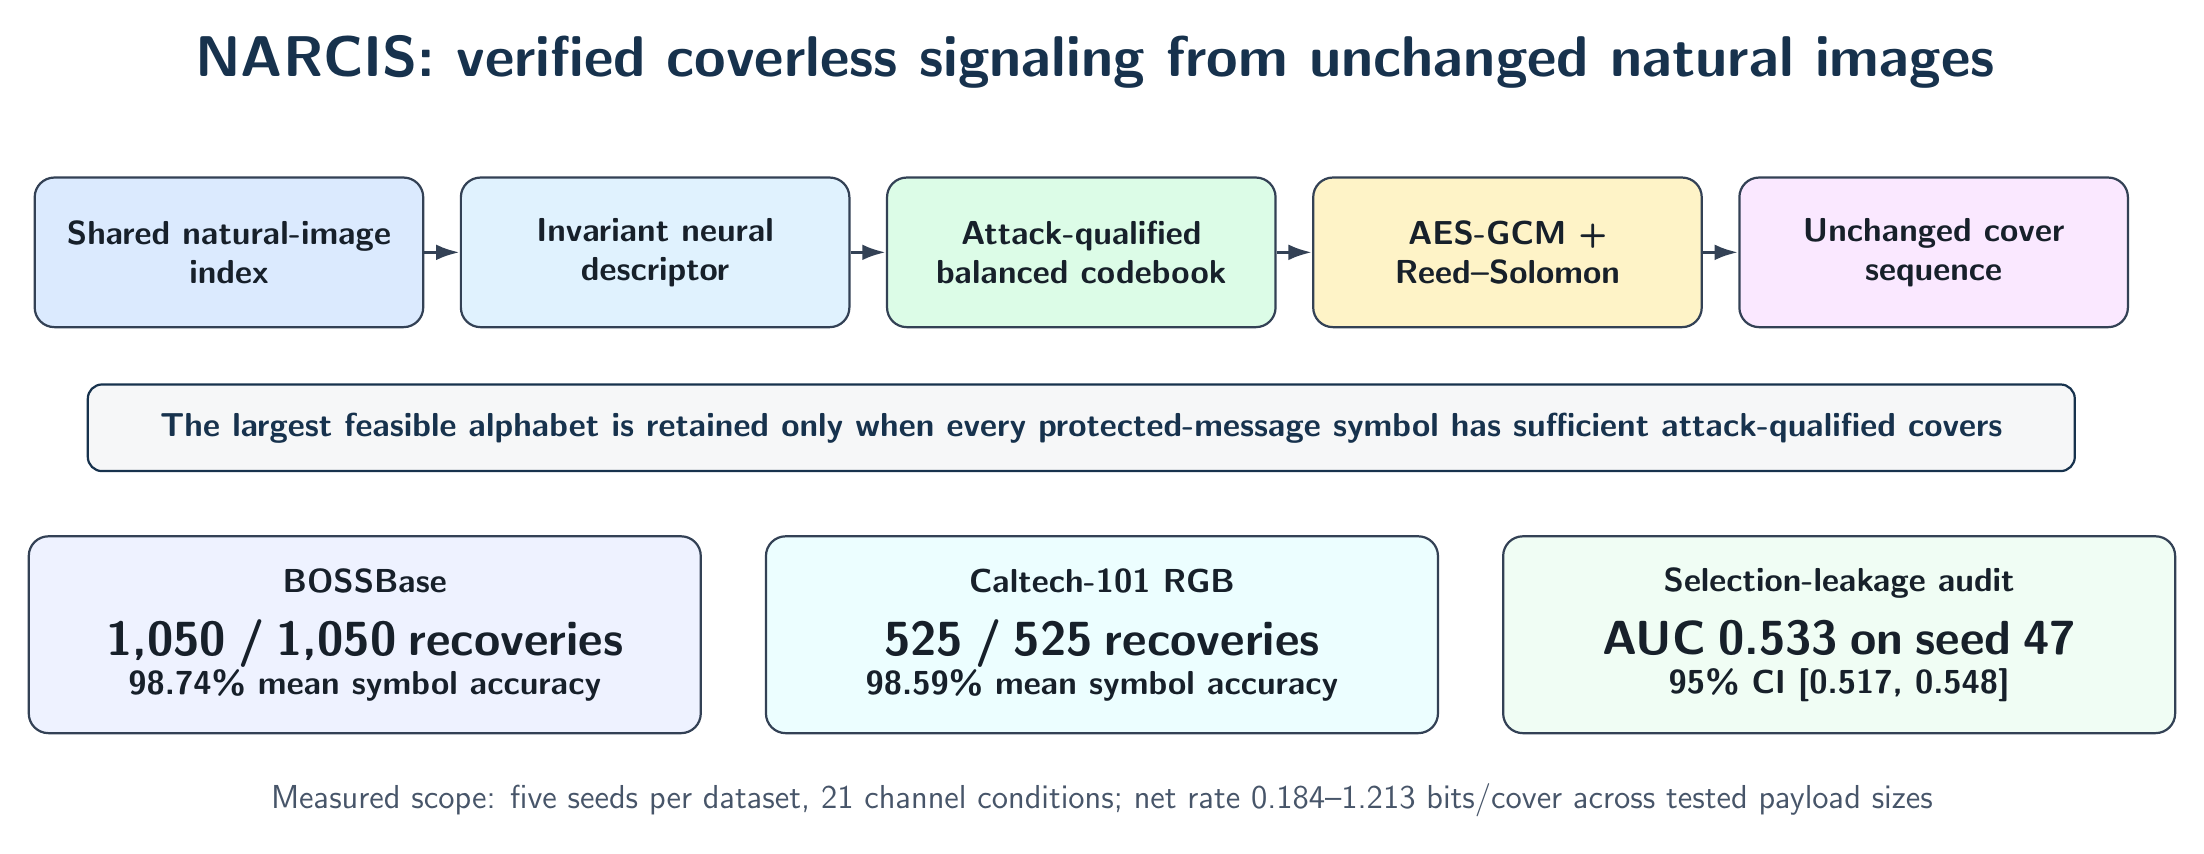
\begin{tikzpicture}[
  font=\sffamily,
  node distance=4.5mm,
  flow/.style={
    draw=line, line width=0.8pt, rounded corners=2.5mm,
    align=center, minimum height=19mm, text width=47mm,
    font=\sffamily\bfseries\large, text=ink
  },
  result/.style={
    draw=line, line width=0.8pt, rounded corners=2.5mm,
    align=center, minimum height=25mm, text width=83mm,
    font=\sffamily\bfseries\large, text=ink
  },
  arrow/.style={-{Latex[length=3mm,width=2mm]}, line width=1.3pt, draw=line}
]

\node[font=\sffamily\bfseries\fontsize{22}{24}\selectfont, text=navy]
  (title) {NARCIS: verified coverless signaling from unchanged natural images};

\node[flow, fill=blueA, below=10mm of title, xshift=-110mm]
  (index) {Shared natural-image\\index};
\node[flow, fill=blueB, right=of index]
  (descriptor) {Invariant neural\\descriptor};
\node[flow, fill=greenA, right=of descriptor]
  (codebook) {Attack-qualified\\balanced codebook};
\node[flow, fill=goldA, right=of codebook]
  (protection) {AES-GCM +\\Reed--Solomon};
\node[flow, fill=violetA, right=of protection]
  (sequence) {Unchanged cover\\sequence};

\draw[arrow] (index) -- (descriptor);
\draw[arrow] (descriptor) -- (codebook);
\draw[arrow] (codebook) -- (protection);
\draw[arrow] (protection) -- (sequence);

\node[
  below=7mm of codebook,
  draw=navy, line width=0.8pt, rounded corners=1.8mm,
  fill=navy!4, text=navy, text width=250mm, minimum height=11mm,
  align=center, font=\sffamily\bfseries\large
] (rule) {The largest feasible alphabet is retained only when every protected-message
symbol has sufficient attack-qualified covers};

\node[result, fill=resultA, below=8mm of rule, xshift=-91mm]
  (boss) {BOSSBase\\[1mm]
  \fontsize{18}{20}\selectfont 1,050 / 1,050 recoveries\\
  \large 98.74\% mean symbol accuracy};
\node[result, fill=resultB, right=8mm of boss]
  (caltech) {Caltech-101 RGB\\[1mm]
  \fontsize{18}{20}\selectfont 525 / 525 recoveries\\
  \large 98.59\% mean symbol accuracy};
\node[result, fill=resultC, right=8mm of caltech]
  (audit) {Selection-leakage audit\\[1mm]
  \fontsize{18}{20}\selectfont AUC 0.533 on seed 47\\
  \large 95\% CI [0.517, 0.548]};

\node[
  below=5mm of caltech, text=muted, align=center,
  font=\sffamily\fontsize{13}{15}\selectfont
] (scope) {Measured scope: five seeds per dataset, 21 channel conditions;
net rate 0.184--1.213 bits/cover across tested payload sizes};

\end{tikzpicture}
\end{document}
